\documentclass[oneside, 11pt]{article}

\usepackage[T1]{fontenc}
\usepackage[utf8]{inputenc}
\usepackage[english]{babel}

\usepackage{fouriernc}
\usepackage[detect-all, binary-units, separate-uncertainty=true,
            per-mode=symbol, retain-explicit-plus, retain-unity-mantissa=false]{siunitx}

\usepackage{setspace}
\setstretch{1.2}

\setlength{\parskip}{\smallskipamount}
\setlength{\parindent}{0pt}

\usepackage[headheight=14pt]{geometry}
\geometry{marginparwidth=0.5cm, verbose, a4paper, tmargin=3cm, bmargin=3cm,
          lmargin=2cm, rmargin=2cm}

\usepackage{float}

\usepackage[fleqn]{amsmath}
\numberwithin{equation}{section}
\numberwithin{figure}{section}

\usepackage{graphicx}
\graphicspath{{images/}{../../../images/}}

\usepackage{tikz}
\usetikzlibrary{shapes}
\usetikzlibrary{plotmarks}

\newcounter{Exercise}
\setcounter{Exercise}{1}
\usepackage{xcolor}
\definecolor{shadecolor}{gray}{0.9}
\usepackage{framed}
\usepackage{caption}

\usepackage{url}


\usepackage{fancyhdr}
\pagestyle{fancy}
\fancyhf{}
\rhead{\thepage}
\renewcommand{\footrulewidth}{0pt}
\renewcommand{\headrulewidth}{0pt}

\fancypagestyle{firststyle}
{
    \fancyhf{}
    \rhead{\thepage}
    \cfoot{
\includegraphics[height=30pt]{HiSPARClogo}}
    \rfoot{
\includegraphics[height=25pt]{CCbysa}}
    \lfoot{
\includegraphics[height=30pt]{NIKHEFlogo}}
    \renewcommand{\footskip}{50pt}
    \renewcommand{\footrulewidth}{0.1pt}
    \renewcommand{\headrulewidth}{0pt}
}

\newcommand{\figref}[1]{Figuur~\ref{#1}}

\newcommand{\hisparc}{\textsmaller{HiSPARC}\xspace}
\newcommand{\kascade}{\textsmaller{KASCADE}\xspace}
\newcommand{\sapphire}{\textsmaller{SAPPHiRE}\xspace}
\newcommand{\jsparc}{\textsmaller{jSparc}\xspace}
\newcommand{\hdf}{\textsmaller{HDF5}\xspace}
\newcommand{\aires}{\textsmaller{AIRES}\xspace}
\newcommand{\csv}{\textsmaller{CSV}\xspace}
\newcommand{\python}{\textsmaller{PYTHON}\xspace}
\newcommand{\corsika}{\textsmaller{CORSIKA}\xspace}
\newcommand{\labview}{\textsmaller{LabVIEW}\xspace}
\newcommand{\daq}{\textsmaller{DAQ}\xspace}
\newcommand{\adc}{\textsmaller{ADC}\xspace}
\newcommand{\hi}{\textsc{h i}\xspace}
\newcommand{\hii}{\textsc{h ii}\xspace}
\newcommand{\mip}{\textsmaller{MIP}\xspace}
\newcommand{\hisparcii}{\textsmaller{HiSPARC II}\xspace}
\newcommand{\hisparciii}{\textsmaller{HiSPARC III}\xspace}

\DeclareSIUnit{\electronvolt}{\ensuremath{\mathrm{e\!\!\:V}}}

\DeclareSIUnit{\unitsigma}{\ensuremath{\sigma}}
\DeclareSIUnit{\mip}{\textsmaller{MIP}}
\DeclareSIUnit{\adc}{\textsmaller{ADC}}

\DeclareSIUnit{\gauss}{G}
\DeclareSIUnit{\parsec}{pc}
\DeclareSIUnit{\year}{yr}





%document details
\author{J. Kortland \\ translated and adapted by K. Schadenberg}
\date{}
\title{Stellar Evolution}


\begin{document}
\maketitle

\section{Introduction}
The origins of high energy cosmic radiation are still unknown. Possible sources are, amongst others, supernovae, black holes, and quasars. A supernova and a black hole are two different end stages of the life of a (large and heavy) star. This module briefly explains the life cycle of a star, from the beginnings as a protosolar nebula to the end stages as a black dwarf or black hole.

\subsection{Types of Stars}
The evolution of stars can be visualised in two different ways. The first is by arranging all the stars in a large diagram according to their colour, on the vertical axis, and their brightness, on the horizontal axis. The obtained diagram is called the Hertzsprung-Russell-diagram, HRD for short. See figure~\ref{fig:HRD_1} for an example.

\begin{figure}\begin{center}
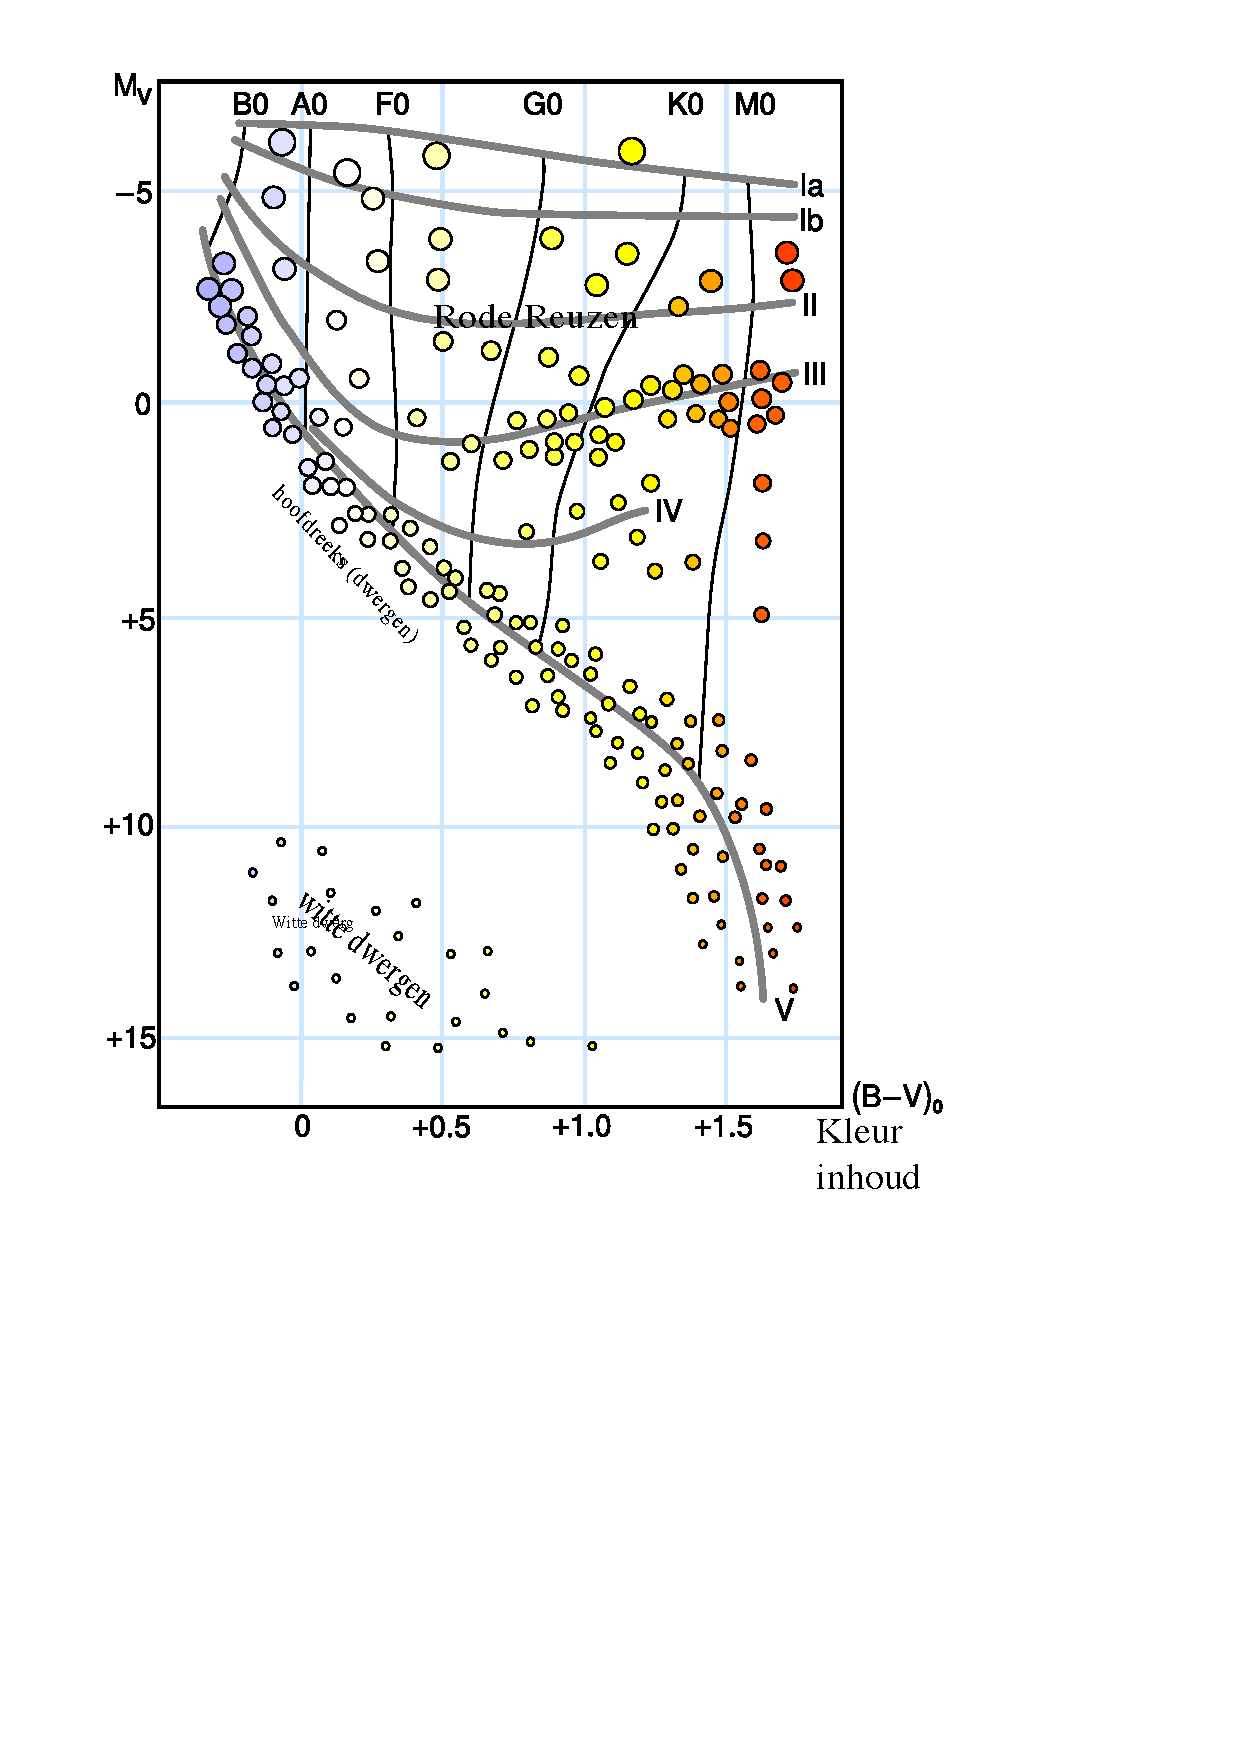
\includegraphics[scale=0.4]{H-R_diagram}
\caption{Stellar classification according in a Hertzsprung-Russell diagram.\protect\footnotemark}\label{fig:HRD_1}
\end{center}\end{figure}
\footnotetext{Picture taken from \url{http://en.wikipedia.org/wiki/File:H-R_diagram.svg}}

Stars are not spread out evenly across the entire diagram, they form clusters in certain areas. The most dense area of the HRD is the main sequence and roughly follows the diagonal. The stars in this sequence are `burning' hydrogen and turning it into helium. The rate at which this happens depends on the location of the star on the diagonal. Small red stars (bottom right) spend tens of billions of years in the main sequence. Our Sun, which is located roughly halfway, only remains in the main sequence for roughly ten billions years. More massive stars such as Sirius (slightly above the Sun) and the blue giant Rigel (top left) spend even less time in the main sequence, half a billions and a couple of millions years respectively.

The second dense area in the HRD can be found in the top right. Here we find the red giants and red super giants such as Betelgeuse, Antares, and Aldebaran. These stars are heavier than our Sun and are `burning' helium to form carbon, oxygen or even heavier elements.

To the left of the red giants we find the horizontal branch. Here lighter stars, such as our Sun, perform the transformation of helium to heavier elements. Even further to the left are the planetary nebulas. Making a sharp turn to the left (downward in the diagram) we end up in the area of the white dwarfs.

\subsection{The Life of a Star}
The second way of looking at the evolution of a star is by plotting its course through the HRD. This is done in figure~\ref{fig:HRD_2} for a star like our Sun. The exact route the star takes and at which speed depends on the mass of the star.

\begin{figure}\begin{center}
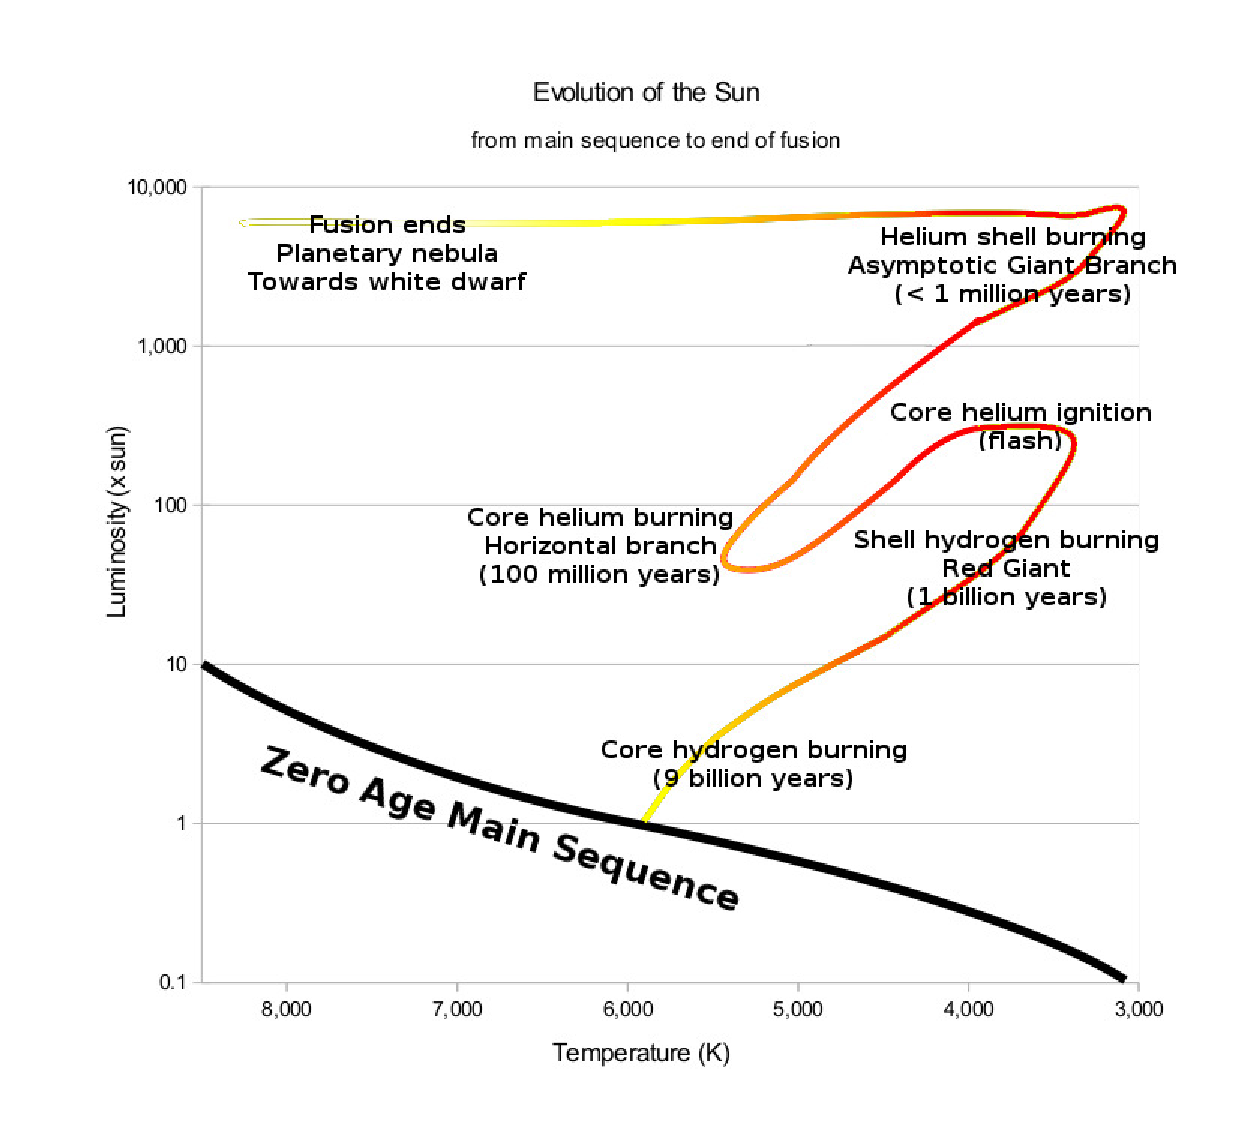
\includegraphics[scale=0.7]{Evolution_of_a_sun-like_star}
\caption{Evolutionary phases of a Sun like star beginning in the main sequence.\protect\footnotemark}\label{fig:HRD_2}
\end{center}\end{figure}
\footnotetext{Picture taken from \url{http://en.wikipedia.org/wiki/File:Evolution_of_a_sun-like_star.png}}

Shortly after their formation inside vast condensing interstellar clouds, bright red stars, stars of the T Tauri type, move towards the left hand side of the graph where they encounter the main sequence. Here they stay until their central supply of hydrogen is depleted. Then they start moving to the right hand side of the diagram. The exact direction depends on the mass of the star. Stars heavier than our Sun will start helium fusion amongst the red giants. But the fusion process does not stop here for these stars, they are massive enough to fuse even larger atoms together. The heaviest stars in this group can reach temperatures of four or even five billions degrees kelvin. Their life will end with an explosion due to these enormous temperatures, a supernova. 

Stars with a mass similar to or lighter than our Sun will spend only a part of their life as a red giant. They will follow the horizontal branch to live amongst the planetary nebulas, pass round behind the main sequence and down towards the white dwarfs. They will continue to slips towards the bottom of the diagram where they end up amongst the stars who have spend all of their fusion fuel: the black dwarfs.

\subsection{Black Holes}
When a star with a large mass dies it both explodes and implodes. The outer layers of the star explode forming a supernova, hurtling large amounts of particles into space. The inner layers implode, they collapse inward due to the large gravitational forces. During this implosion a black hole might be created. The mass in concentrated so densely that the escape velocity at the surface is larger than 300,000~km/s, preventing even light from escaping. Another possible origin of black holes might be the early stages of our Universe in which there were also very dense concentrations of matter.

How can we observe, `see', a black hole? We cannot look for any radiation coming from the black holes, as we do with other celestial bodies, because it cannot escape. Instead we look for the signs of the large gravitational field created by the black hole. This field has a very specific effect on the radiation coming from binary stars and quasars. From Earth we can, with the right tools, observe a large number of binary stars. Binary or `double' stars are pairs of two stars very close to each other and orbiting each other. The barycentre, the point around which both stars seem to rotate, will lie somewhere between the two stars. If one of the stars is a black hole however, we will only see one star which rotates around a point in space. Astronomers already observed a few possible such binary stars.

\subsubsection{Quasars}
Amongst all the galaxies (systems of stars, remnants of stars, and interstellar medium of gas and dust) quasars are the strongest sources of radiation we know. One quasar can be as `bright' as a thousand ordinary galaxies, or one hundred thousand billion times as bright as our Sun. The source of all this radiation is concentrated in a small area, no larger than our solar system, at the centre of the galaxy. What mechanism can produce and emit such large quantities of radiation while being contained to such a small volume? One possibility is a black hole with a mass a few million times larger than our Sun.

This may seem strange, paradoxical even, because we said earlier that not even light can escape a black hole. To explain what happens we need to look at what a black holes does. Because of its large mass the black hole will pull everything towards itself using gravity. Everything that comes too close will be devoured by the black hole, be it dust clouds, planets, or even stars. When these object `fall' towards the black hole their velocity increases, they accelerate. During their fall they collide with other objects at high speed. These collisions create the massive amounts of radiation.

\subsubsection{Disappearing Black Holes?}
Black holes seem to be full of surprises. The English astrophysicist Stephen Hawking postulated that black holes can slowly `evaporate'. Again a paradox because nothing can escape from a black hole. The exact details involve a large amount of quantum mechanics and are beyond the scope of this text. But if Hawking is right the evaporation of a black hole will decrease its mass which in turn will speed up the evaporation. This process ends in a large explosion that emits such a large amount of radiation that is should be visible billions of light years away.

\begin{shaded}
\textbf{Exercise \theExercise \stepcounter{Exercise}} : The HRD can be seen as the path a star walks during his life. To determine the location of a star in the HRD we need to know its absolute magnitude or luminosity and surface temperature. How does an astronomer determine these values? Do a bit of online research to answer this question.\end{shaded}

\begin{shaded}
\textbf{Exercise \theExercise \stepcounter{Exercise}} : The different stages in the life of a star are connected to fusion reaction taking place inside the star. Can you further explain this connection? Do a bit of online research to answer this question.\end{shaded}

\end{document}


\begin{shaded}
\textbf{Exercise \theExercise \stepcounter{Exercise}} : \end{shaded}

\footnotemark
\footnotetext{}

